% Chapter 7

\chapter{Experimental Results} % Main chapter title

\label{Chapter7} % For referencing the chapter elsewhere, use \ref{Chapter1} 

\lhead{Chapter 7. \emph{Experimental Results}}

%----------------------------------------------------------------------------------------

All the experimental data is available in an Excel file at \url{https://github.com/HL-Boisvert/MSc_Project_HW}. The data was extracted from ROS using the data scripts in the \verb|Wall Following| and \verb|DQN| folders and has been processed to be easily understandable. Spreadsheets for answering the hypotheses were also included in the Excel file.

\section{Experimental Requirements E3 and E5}
\label{exp_assessment}
Experimental Requirement E3 consisted of assessing the performance of the Wall Following controller according to the updated metrics on the four simulated tracks. \\
Regarding Experimental Requirement E5 (DQN assessment), as explained in the GitHub repository, all 6 controllers were trained for 1 million steps (around 20h), using the same hyper-parameters. Values replaced with ``\verb|/|" indicate that the lap couldn't be completed by the car. \\
It was decided to compare the performance of all controllers one track at a time:
Tables \ref{redbull_results}, \ref{monaco_results}, \ref{silverstone_results} and \ref{oval_results} introduce the results for each track; the detailed data is available in the Excel file. \\

\begin{table}
\centering
\begin{tabularx}{\textwidth}{||X|X|X|X|X|X|X||} 
\hline
 Controller & Total Time ($s$) & Average Positive Acceleration ($m/s^2$)& Average Negative Acceleration ($m/s^2$) & Maximum Acceleration ($m/s^2$) & Maximum Deceleration ($m/s^2$) & Average Minimum LiDAR Range ($m$)\\ [0.5ex] 
 \hline\hline
Wall Following & 26.86 & 1.17 & -3.16 & 4.87 & -7.90 & 0.84\\[0.5ex] 
 \hline
 NN R1 & 36.24 & 1.00 & -3.61 & 5.39 & -6.51 & 0.84\\[0.5ex] 
 \hline
 NN R2 & 27.81 & 1.31 & -3.35 & 5.09 & -5.81 & 0.82\\[0.5ex] 
 \hline
NN R3 & 29.15 & 0.82 & -4.54 & 3.49 & -6.71 & 0.81\\[0.5ex] 
 \hline
 CNN R1 & 35.24 & 0.82 & -3.48 & 6.35 & -5.57 & 0.81\\[0.5ex] 
 \hline
 CNN R2 & 25.17 & 0.72 & -3.23 & 4.97 & -6.72 & 0.80\\[0.5ex] 
 \hline
 CNN R3 & 24.20 & 1.09 & -2.23 & 5.38 & -6.53 & 0.77\\[0.5ex] 
 \hline
\end{tabularx}
\caption{Experimental results on the RedBull track}
\label{redbull_results}
\end{table}

\begin{table}
\centering
\begin{tabularx}{\textwidth}{||X|X|X|X|X|X|X||} 
\hline
 Controller & Total Time ($s$) & Average Positive Acceleration ($m/s^2$)& Average Negative Acceleration ($m/s^2$) & Maximum Acceleration ($m/s^2$) & Maximum Deceleration ($m/s^2$) & Average Minimum LiDAR Range ($m$)\\ [0.5ex] 
 \hline\hline
Wall Following & 50.68 & 1.10 & -2.41 & 3.59 & -7.90 & 0.84\\[0.5ex] 
 \hline
 NN R1 & / & / & / & / & / & /\\[0.5ex] 
 \hline
 NN R2 & 53.62 & 0.87 & -3.73 & 5.61 & -6.69 & 0.77\\[0.5ex] 
 \hline
NN R3 & 56.34 & 0.81 & -3.55 & 4.71 & -2.90 & 0.80\\[0.5ex] 
 \hline
 CNN R1 & / & / & / & / & / & /\\[0.5ex] 
 \hline
 CNN R2 & 46.74 & 0.90 & -1.29 & 5.24 & -6.58 & 0.78\\[0.5ex] 
 \hline
 CNN R3 & 45.01 & 0.88 & -1.09 & 4.31 & -2.91 & 0.78\\[0.5ex] 
 \hline
\end{tabularx}
\caption{Experimental results on the Monaco track}
\label{monaco_results}
\end{table}


\begin{table}
\centering
\begin{tabularx}{\textwidth}{||X|X|X|X|X|X|X||} 
\hline
 Controller & Total Time ($s$) & Average Positive Acceleration ($m/s^2$)& Average Negative Acceleration ($m/s^2$) & Maximum Acceleration ($m/s^2$) & Maximum Deceleration ($m/s^2$) & Average Minimum LiDAR Range ($m$)\\ [0.5ex] 
 \hline\hline
Wall Following & 51.92 & 0.89 & -3.11 & 4.06 & -7.52 & 0.65\\[0.5ex] 
 \hline
 NN R1 & / & / & / & / & / & /\\[0.5ex] 
 \hline
 NN R2 & 61.22 & 2.43 & -1.21 & 4.61 & -5.22 & 0.81\\[0.5ex] 
 \hline
NN R3 & 63.41 & 1.22 & -1.57 & 5.24 & -6.79 & 0.80\\[0.5ex] 
 \hline
 CNN R1 & / & / & / & / & / & /\\[0.5ex] 
 \hline
 CNN R2 & 49.78 & 1.01 & -2.13 & 5.79 & -5.48 & 0.81\\[0.5ex] 
 \hline
 CNN R3 & 50.44 & 0.86 & -1.43 & 4.59 & -4.83 & 0.78\\[0.5ex] 
 \hline
\end{tabularx}
\caption{Experimental results on the Silverstone track}
\label{silverstone_results}
\end{table}


\begin{table}
\centering
\begin{tabularx}{\textwidth}{||X|X|X|X|X|X|X||} 
\hline
 Controller & Total Time ($s$) & Average Positive Acceleration ($m/s^2$)& Average Negative Acceleration ($m/s^2$) & Maximum Acceleration ($m/s^2$) & Maximum Deceleration ($m/s^2$) & Average Minimum LiDAR Range ($m$)\\ [0.5ex] 
 \hline\hline
Wall Following & 3.80 & 1.23 & -4.04 & 4.90 & -7.51 & 0.62\\[0.5ex] 
 \hline
 NN R1 & 3.26 & 1.31 & -0.87 & 3.51 & -1.73 & 0.76\\[0.5ex] 
 \hline
 NN R2 & 3.19 & 1.22 & -0.96 & 3.40 & -1.93 & 0.81\\[0.5ex] 
 \hline
NN R3 & 2.98 & 1.21 & -0.96 & 4.51 & -1.62 & 0.78\\[0.5ex] 
 \hline
 CNN R1 & 3.01 & 1.36 & -0.51 & 3.82 & -1.89 & 0.78\\[0.5ex] 
 \hline
 CNN R2 & 3.42 & 1.21 & -1.82 & 2.98 & -1.25 & 0.79\\[0.5ex] 
 \hline
 CNN R3 & 2.95 & 1.26 & -0.74 & 3.91 & -1.42 & 0.78\\[0.5ex] 
 \hline
\end{tabularx}
\caption{Experimental results on the oval track}
\label{oval_results}
\end{table}

To answer Hypothesis n°3, the CNNs trained on the Monaco Track were then compared to those trained on the RedBull track when racing on the Monaco Track; the results for all metrics are introduced in Table \ref{hyp3}.

\begin{table}
\centering
\begin{tabularx}{\textwidth}{||X|X|X|X|X|X|X||} 
\hline
 Controller & Total Time ($s$) & Average Positive Acceleration ($m/s^2$)& Average Negative Acceleration ($m/s^2$) & Maximum Acceleration ($m/s^2$) & Maximum Deceleration ($m/s^2$) & Average Minimum LiDAR Range ($m$)\\ [0.5ex] 
 \hline\hline
 CNN R2 Monaco Trained & 42.28 & 0.93 & -1.25 & 5.18 & -6.67 & 0.80\\[0.5ex] 
 \hline
 CNN R3 Monaco Trained & 40.91 & 0.84 & -1.14 & 4.34 & -2.69 & 0.83\\[0.5ex] 
 \hline
CNN R2 RedBull Trained & 46.74 & 0.90 & -1.29 & 5.24 & -6.58 & 0.78\\[0.5ex] 
 \hline
 CNN R3 RedBull Trained & 44.98 & 0.89 & -1.10 & 4.30 & -2.94 & 0.77\\[0.5ex] 
 \hline
 \end{tabularx}
\caption{Experimental results on the Monaco Track comparing DQN controllers trained on Monaco or RedBull tracks}
\label{hyp3}
\end{table}


\section{Experimental Requirement E8}
Experimental Requirement E8 consisted of running the Wall Following and DQN controllers on the physical car, racing on the oval race track built using flexible tubes, with the goal of evaluating the Sim2Real gap. It was found that the height of a single flexible tube was not enough to be reliably detected by the LiDAR. Thus, a second perimeter of tubes had to be taped on top of the first one (Figure \ref{track}).

\begin{figure}
\centering
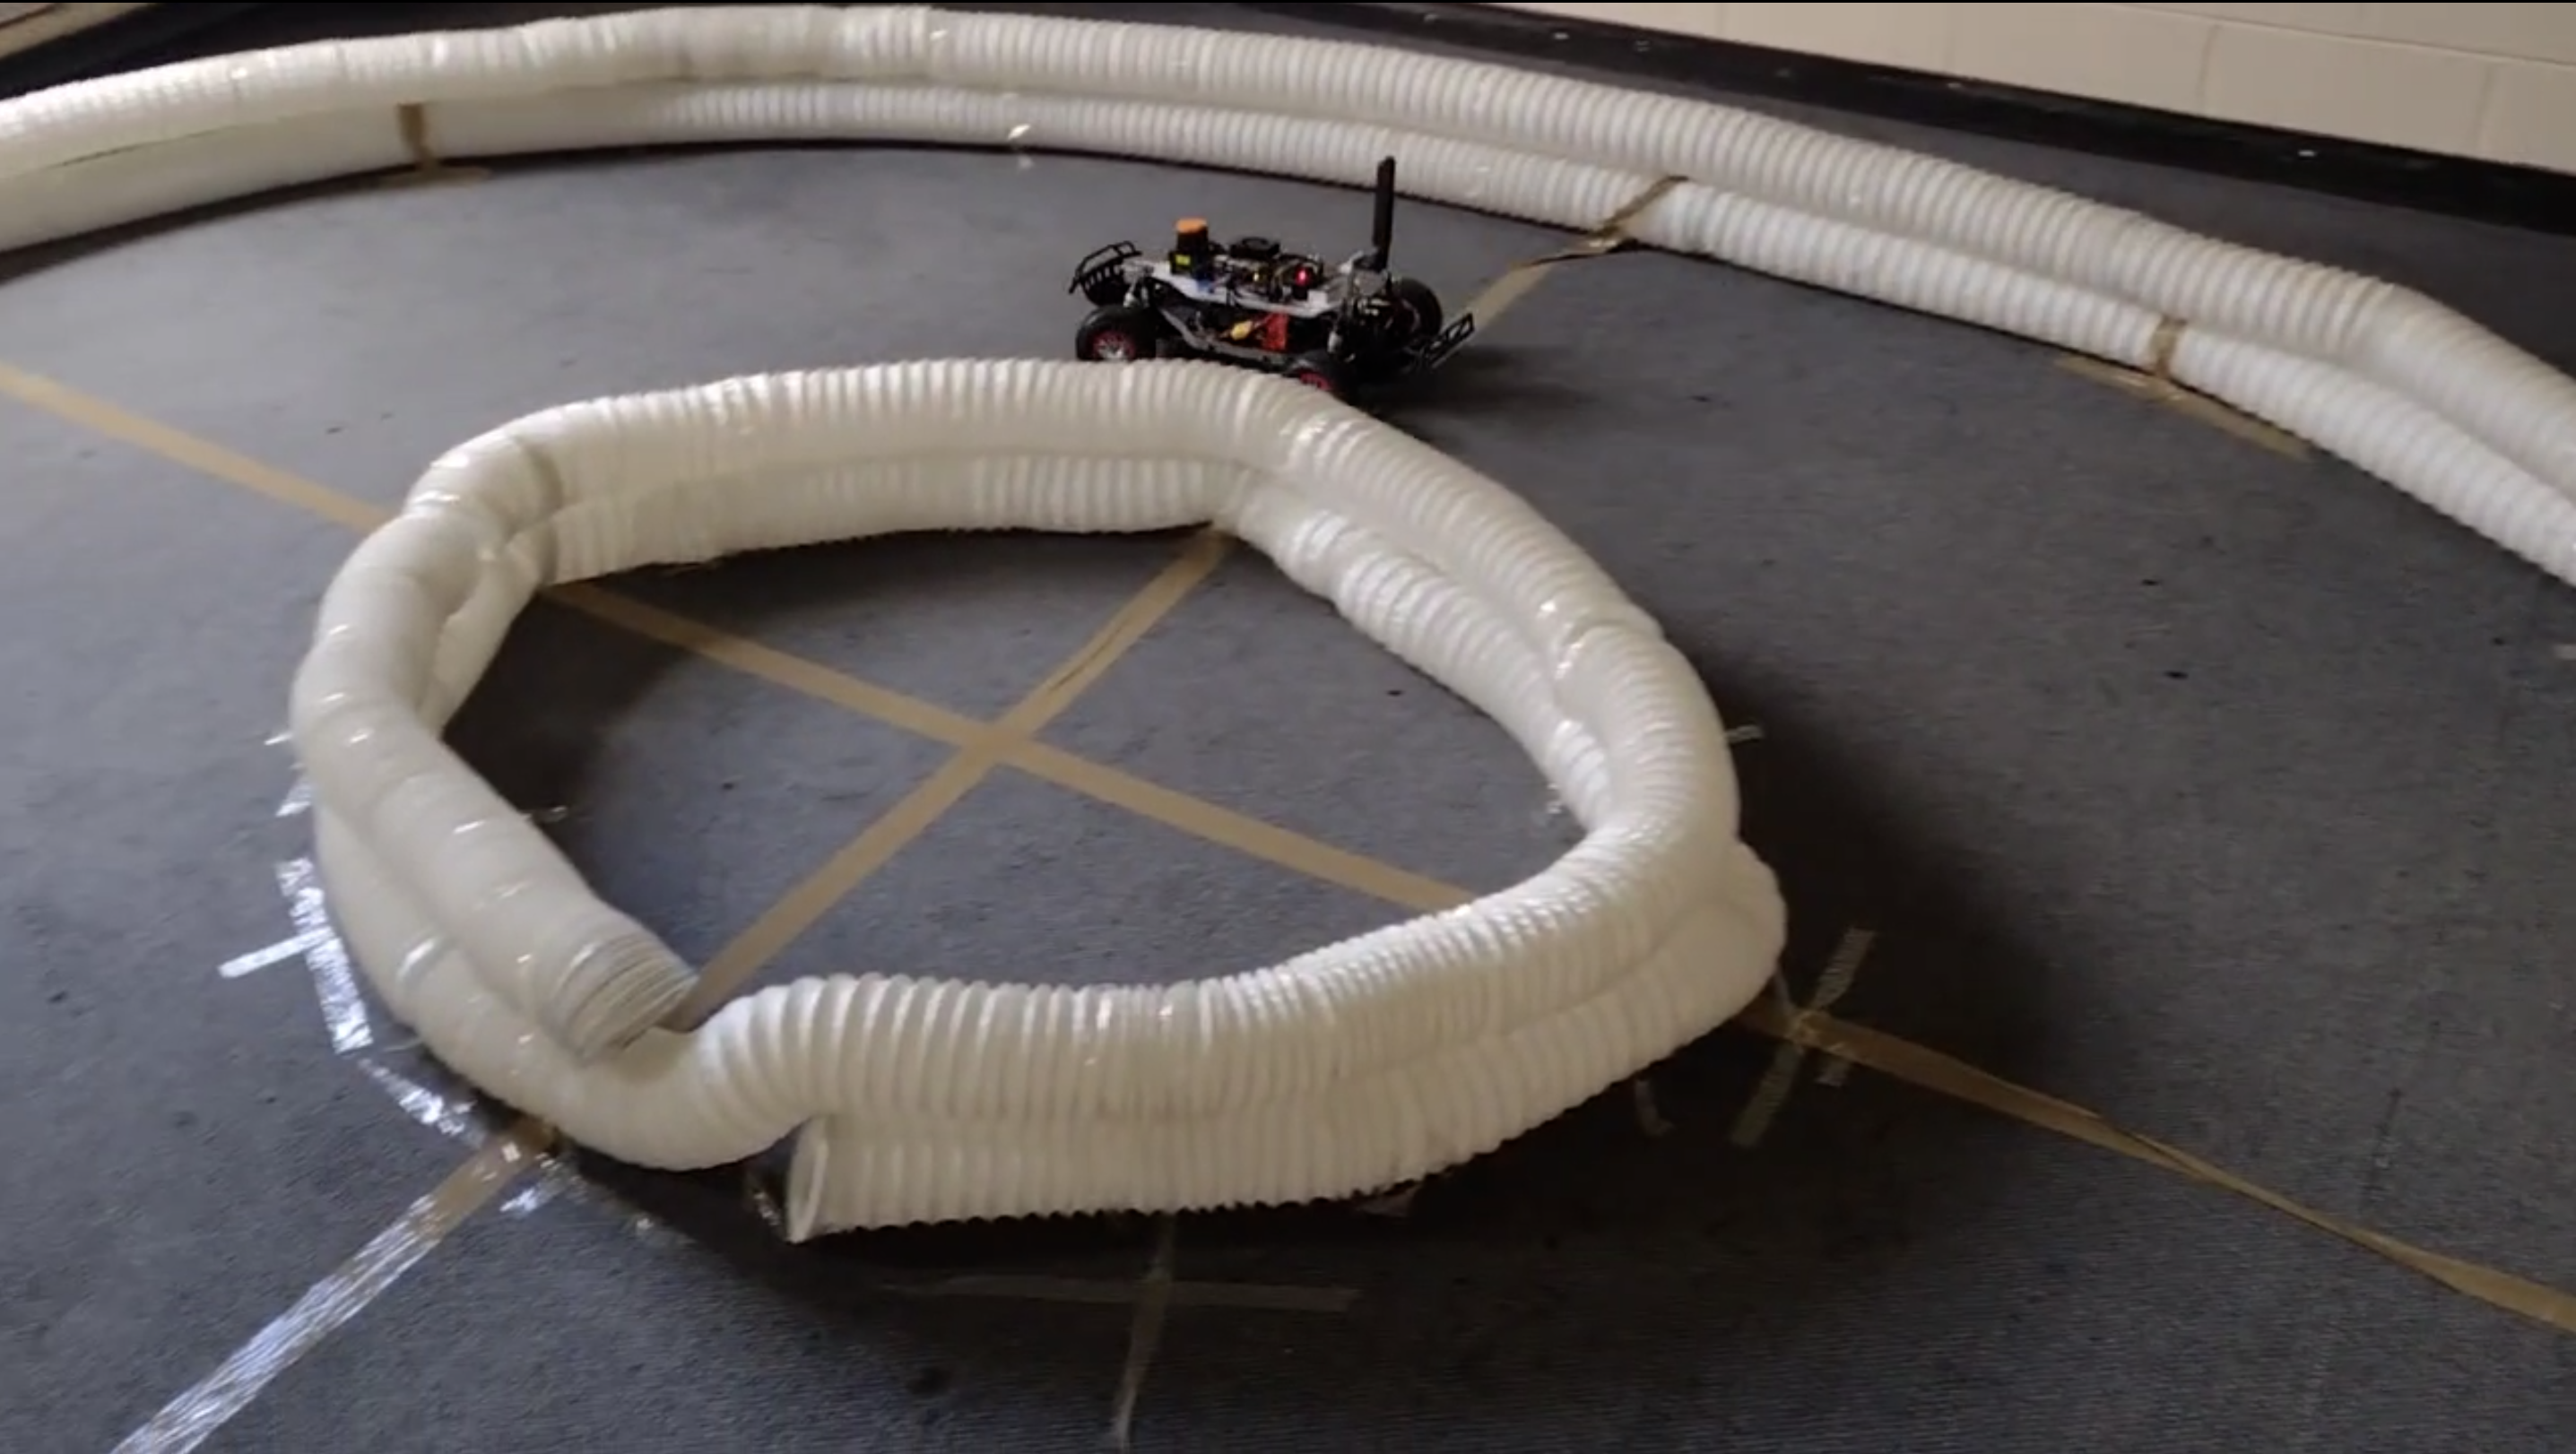
\includegraphics[scale=0.12]{Figures/track.png}
\caption{Track with the car in starting position}
\label{track}
\end{figure}

\subsection{Wall Following controller}
It quickly appeared that the tuning of the gains $k_p$, $k_d$, and $k_i$ in the simulator was not adapted to the physical car, which showed a clear Sim2Real gap; the PID was tuned again in the same way as explained in Chapter \ref{Chapter6}, and detailed results are available in the Excel file. It also appeared the controller was not performing properly at a speed of 5 m/s: the max speed was changed to 4 m/s, and the simulator experiments were performed again with the new max speed. 
\subsection{DQN}
The same problem was encountered on the car when installing TensorFlow on the Jetson and was solved by following the instructions at \url{https://docs.nvidia.com/deeplearning/frameworks/install-tf-jetson-platform/index.html}. \\
After some testing, it was found the odometry wasn't reliable and couldn't be used as input for the NN and CNN controllers, meaning new controllers had to be trained. Because of time constraints, only the most performant controller (CNN with reward function n°3) was retrained. Because the odometry couldn't be relied upon, the metrics that depended on the speed measurement couldn't be assessed, which only left the lap time and average minimal LiDAR distance metrics; this was considered enough to answer Hypothesis n°4. \\
Finally, there was an issue with the controller in the last turn of the lap which made the car collide with the tubes; the issue happened each time a lap was attempted, even when adding a higher obstacle and changing the lighting in the room. In the end, it was decided to use the data only on 3 quarters of a lap and then extrapolate. The problem couldn't really be explained, it may be linked to the training data, the LiDAR input, the hardware itself or several of those reasons at the same time. \\
The detailed data is available in the Excel file, and the main results are introduced in Table \ref{hyp4} (averages over 3 laps). 

\begin{table}[H]
\centering
\begin{tabularx}{\textwidth}{||X|X|X|X|X|X|X||} 
\hline
 Controller & Total Time ($s$) & Average Minimum LiDAR Range ($m$)\\ [0.5ex] 
 \hline\hline
 Manual Driving & 5.47 & 0.72 \\[0.5ex] 
 \hline
 Wall Following & 3.75 & 0.76\\[0.5ex] 
 \hline
CNN RW3 & 3.55 & 0.77\\[0.5ex] 
 \hline
\end{tabularx}
\caption{Experimental results on the physical oval track}
\label{hyp4}
\end{table}
